\chapter{English-German}
\label{chap:german}

In this chapter we are going to describe changes we have made to an existing
English-Czech MLFix pipeline to be able to apply the system to the English-German
SMT outputs. We are going to summarize the data available for training the models
and evaluate the system in the system in a similar way we did with the English-Czech
pipeline.

\section{Processing pipeline modification}

As we have mentioned, we have focused on making the processing pipeline as independent
on the target language as possible. However, we still have to replace some of the tools
used for the Czech analysis to be able to correctly process German sentences.

Again, we have used the Treex framework as a backbone of the processing pipeline and
necessary 3rd party tools were implemented into the systems via wrappers.
After the sentences are read in parrallel, they are processed separately, English
following the same scenario as in the English-Czech pipeline.
German is again tokenized, this time by a set of regex rules inspired by Tiger corpus\cite{Brants2004}
with main focus on abbreviations, ordinal numbers and compounds connected by hyphens.

Next, lemmatization and POS tagging is performed by a Mate tools\footurl{http://www.ims.uni-stuttgart.de/forschung/ressourcen/werkzeuge/matetools.en.html}
toolkit. The tagger used CoNLL2009\cite{CoNLL-2009-ST} tagset. For tagging, we could have also
used the Stanford POS Tagger\footurl{http://nlp.stanford.edu/software/tagger.shtml}\cite{Toutanova:2000:EKS:1117794.1117802},
however, the tagset it uses contains only coarse tags without little morphological information.
To convert the CoNLL2009 tags to Interset, we use a decoder, which was already implemented at the
time of our research.

For the word alignment, we again use GIZA++. Similar to English-Czech, we produce one-to-one word alignment
with the intersetion symmetrization. We The alignment model has been trained on the European
Parliament Parallel corpus\cite{koehn2005epc}\footnote{http://www.statmt.org/europarl/} (Europarl)
containing nearly two million sentences. During the process of training data analysis we 
also create monolingual alignment between the MT output and the references sentences
in a similar way we did in the original pipeline.

The dependency structure for the MT output is again produced by projecting the English dependency
structures on the MT sentences. When processing the training data, we parse the reference sentences
by graph-based parser\cite{Bohnet:2010:VHA:1873781.1873792} implementation which is also a part of the
Mate tools toolkit. We stop the analysis at the a-layer, but again in the future, further analyzing
the sentences to the t-layer to gain additional features for extraction is desired.

We have reused the statistical component used in the English-Czech pipeline, because it was designed to be
language independent (with the exception of the statistical models). For wordform generation we have
the Flect morphological generation tool mentioned earlier. We have trained the generator on a small
fraction (around one hundred thousand sentences) of the Europarl corpus. The tool is trained on a set
of features based on a combination of lemma$+$Interset producing the inflected word.\todo{training data acc?}

\section{Data analysis}

We have been able to collect only a smaller variety of data for English-German compared to English-Czech
 mostly due to some datasets we mentioned earlier wer simply not available for this language pair. Still, we have been
available to gather following datasets: WMT16, HimL and Autodesk. Note that in case of Autodesk dataset,
the size of English-German is about three times bigger than the size of English-Czech (around 120k sentences).
For this reason, we have decided to include Autodesk dataset into our training data even though it covers
a limited domain.

When extracting the training instances for the statistical component we have followed same scenario
as before, using the same heuristic to identify \equo{incorrect} wordforms. We have also used the Oracle
classifier to gather information about possible improvements this heuristic can bring when applied to German.

We have also performed quick manual evaluation of the output produced by the Oracle classifier by a non-native
German speaker.
We have performed the evaluation on the WMT16 dataset this time because we have thought that medical domain of HimL dataset
would be too difficult for a non-native speaker to evaluate.
Due to limited
resources we have again used only a single annotator for this evaluation task. The evaluator, not being familiar
with the MLFix system, was presented set of instances containing the following: randomly shuffled MT output and Oracle output,
the source English sentence and the German reference translation. The results of the evaluation a shown in the table\todo{ref}
%okec

\begin{table*}[t]
\centering
\small

\begin{tabular}{l|cc|ccc|cc}
  &  Evaluated  &  Changed  &  $+$  &  $-$  &  0  &  Precision  &  Recall  \\
\hline
Oracle  &  800  &  242  &  155  &  42  &  45  &  64.0\%  &  19.3\%  \\
\end{tabular}
\caption{
Results of the the manual evaluation of the ideal system based on the same heuristic
that has been used in the English-Czech pipeline.
}
\label{oracle_de-maneval}
\end{table*}

After the evaluation of our data extraction method we have analyzed the extracted instances and compared them
to the information we have gathered during Czech data analysis. \Fref{iset_de-barplot} shows the frequency of the changed Interset
categories. Again, case was the most changed category among our data followed by gender and number, either as a standalone change or
as a part of a clustered change. This led us to training the category prediction models in a same manner as in the English-Czech
pipeline with exception of the animateness (\pojem{CNGA}) models. To make sure that we can make similar assumptions during
the model training we have also checked distribution of changes per individual POS categories, shown in~\Tref{changes_de-pos}
%okec

\begin{figure}
\centering
  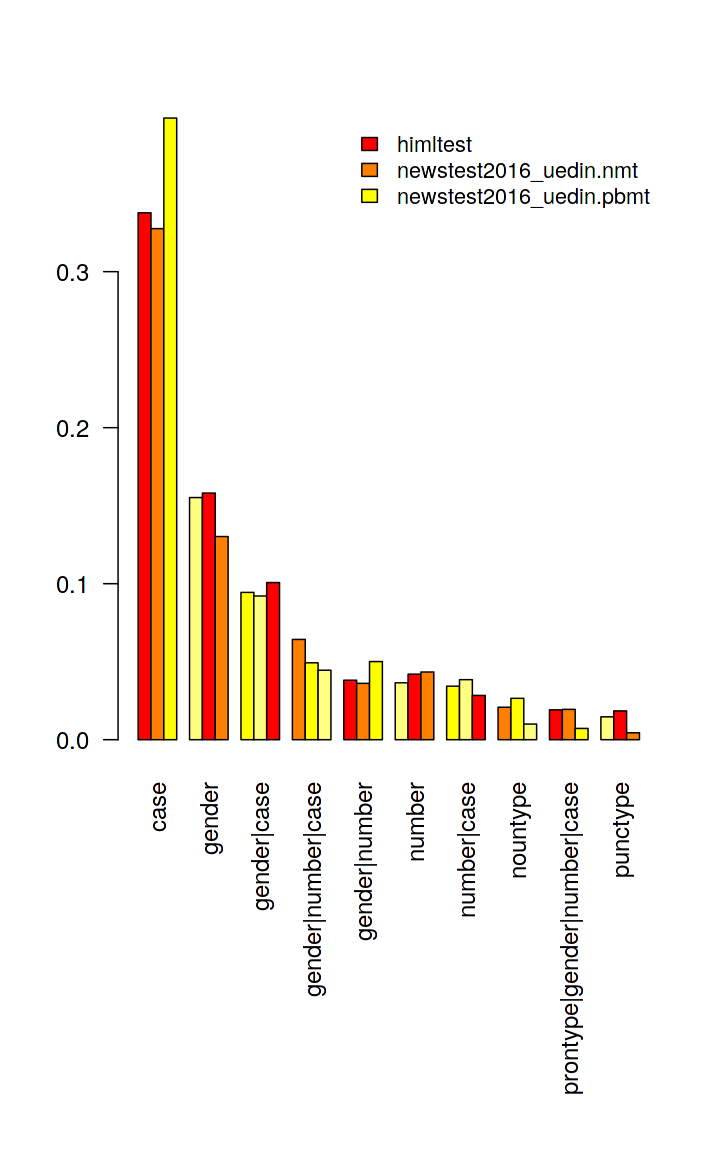
\includegraphics[scale=0.7]{iset_de}
  \caption{
    Frequency of the most changed Interset categories in German data, grouped by a datasets. Categories containing
    "\textbar" symbol (e.g. gender\textbar{}number) represent changes made simultaneously.
}
  \label{iset_de-barplot}
\end{figure}

\begin{table*}[t]
\centering
\small

\begin{tabular}{lc}
POS  &  Frequency  \\
\hline
noun    &   38\%  \\
adj     &   16\%  \\
adp     &   10\%  \\
verb    &   9\%  \\
adv     &   9\%  \\
\end{tabular}
\caption{
    Part-of-speech (POS) frequencies of the changed words.
}
\label{changes_de-pos}
\end{table*}


We

%\todo{avail data?}
\todo{rozbory ala task\_descr?}
%\todo{oracle eval (human)}
